\documentclass[11pt]{article}
\usepackage[margin=1in]{geometry}
\usepackage{amsmath, amssymb, amsthm, esint, physics}
\usepackage{fancyhdr}
\usepackage{tikz, tikz-3dplot}
% \usepackage{hyperref}
\usepackage{enumitem}
\usepackage{caption}
\usepackage{float}

% Page setup
\pagestyle{fancy}
\setlength{\headheight}{14pt}
\fancyhf{}
\lhead{Single Variable Calculus}
\cfoot{\thepage}

\begin{document}
\pagestyle{plain}
\begin{center}
  \tableofcontents
\end{center}
\newpage
\setcounter{page}{1}
\pagestyle{fancy}

\section{Limit}
\subsection{Limit of a Function}
\subsubsection{Definition}
Let $f$ be a function defined on an open interval containing $a$, except possibly at $a$ itself. 
Then \[\lim_{x\to a}f(x) = L\] if for every $\varepsilon > 0$, there exists a $\delta > 0$ such that
\[
0 < |x - a| < \delta \quad \Rightarrow \quad |f(x) - L| < \varepsilon.
\]
\subsubsection{Property}
Let $\displaystyle\lim_{x \to a} f(x) = L$ and $\displaystyle\lim_{x \to a} g(x) = M$, and let $c$ be a constant. Then the following limit properties hold:
\begin{enumerate}
    \item $ 
        \displaystyle
        \lim_{x \to a} [f(x) + g(x)] = L + M
    $    
    \item $
        \displaystyle
        \lim_{x \to a} [f(x) - g(x)] = L - M
    $
    
    \item $
        \displaystyle
        \lim_{x \to a} [c \cdot f(x)] = cL
    $
    
    \item $
        \displaystyle
        \lim_{x \to a} [f(x) \cdot g(x)] = L \cdot M
    $
    
    \item $
        \displaystyle
        \lim_{x \to a} \frac{f(x)}{g(x)} = \frac{L}{M}
    $, \text{if $M \neq 0$}
    
    \item $
        \displaystyle
        \lim_{x \to a} [f(x)]^n = L^n \quad \text{for any } n \in \mathbb{N}
    $
    
    \item $
        \displaystyle
        \lim_{x \to a} \sqrt[n]{f(x)} = \sqrt[n]{L} \quad \text{if } L \ge 0 \text{ for even } n
    $
\end{enumerate}
\subsubsection{One-sided Limit and Existence of a Limit}
Let $f(x)$ be a function defined near $x = a$.\\[.5em]
\textbf{Left-hand limit:}  
$
    \displaystyle
    \lim_{x \to a^-}f(x) = L
$\\
if for every $\varepsilon > 0$, there exists a $\delta > 0$ such that
\[
    0<a-x<\delta\quad\Rightarrow\quad|f(x)-L|<\varepsilon.
\]
\noindent
\textbf{Right-hand limit:}
$
    \displaystyle
    \lim_{x \to a^+} f(x) = L
$\\
if for every $\varepsilon > 0$, there exists a $\delta > 0$ such that
\[
    0<x-a<\delta\quad\Rightarrow\quad|f(x)-L|<\varepsilon.
\]
\textbf{Existence of Limit}\\
The limit of a function $f(x)$ as $x$ approaches $a$ exists if and only if the left-hand and right-hand limits exist and are equal:
\[
    \lim_{x \to a} f(x) \text{ exists } \iff \lim_{x \to a^-} f(x) = \lim_{x \to a^+} f(x)
\]
\subsubsection{Evaluating Limit}
\begin{enumerate}
    \item Substitute directly
    \item Factoring and simplifying
    \item Multiply by the conjugate of numerator or denominator
    \item Use graph/table of a given function
\end{enumerate}
\subsubsection{Squeeze Theorem}
Let $f(x)$, $g(x)$, and $h(x)$ be functions defined on an open interval containing $a$, 
except possibly at $a$ itself. Suppose that for all $x$ in this interval (with $x \ne a$),
\[f(x) \le g(x) \le h(x),\]
and that\[\lim_{x \to a} f(x) = \lim_{x \to a} h(x) = L.\] 
Then,\[\lim_{x \to a} g(x) = L.\]
\bigskip
\noindent
\textbf{For example:}\\
for all $x \ne 0$,
\[
-1 \le \sin\left(\frac{1}{x}\right) \le 1.
\]
Multiplying all parts by $x^2 \ge 0$, we get
\[-x^2 \le x^2 \sin\left(\frac{1}{x}\right) \le x^2.\]
Since
\[\lim_{x \to 0} (-x^2) = 0 = \lim_{x \to 0} x^2,\]
by the \textbf{\textit{Squeeze Theorem}},
\[\lim_{x \to 0} x^2 \sin\left(\frac{1}{x}\right) = 0.\]
\subsection{Limit with Infinities}
\subsubsection{Infinite Limits}
If $f$ is a function defined at every number in some open inverval containing $a$
, except possibly at $a$ itself, then
\begin{itemize}
    \item $\displaystyle\lim_{x \to a} f(x) = \infty$ 
        means that $f(x)$ increases without bound as $x$
        approaches $a$.
    \item $\displaystyle\lim_{x \to a} f(x) = -\infty$ 
        means that $f(x)$ increases without bound as $x$
        approaches $a$.
    
\end{itemize}
\textbf{Limit Theorems}
\begin{enumerate}
    \item If $n$ is a positive integer, then
        \begin{enumerate}
            \item $
                \displaystyle 
                \lim_{x\to0^+}\frac{1}{x^n} = \infty
            $
            \item $
                \displaystyle 
                \lim_{x\to0^-}\frac{1}{x^n} =
                \begin{cases}
                    \infty &\text{if }n\text{ is even}\\
                    -\infty &\text{if }n\text{ is odd}
                \end{cases}
            $
        \end{enumerate}
    \item if the $\displaystyle
        \lim_{x\to a} f(x) =c, c>0, \text{and} \lim_{x\to a} g(x) =0
        \text{, then}$\\$
            \displaystyle\lim_{x\to a}\frac{f(x)}{g(x)}=
        \begin{cases}
            \infty &\text{if }g(x)\text{ approaches 0 through positive values}\\
            -\infty &\text{if }g(x)\text{ approaches 0 through negative values}
        \end{cases}$
    \item if the $\displaystyle
        \lim_{x\to a} f(x) =c, c<0, \text{and} \lim_{x\to a} g(x) =0
        \text{, then}$\\$
            \displaystyle\lim_{x\to a}\frac{f(x)}{g(x)}=
        \begin{cases}
            -\infty &\text{if }g(x)\text{ approaches 0 through positive values}\\
            \infty &\text{if }g(x)\text{ approaches 0 through negative values}
        \end{cases}$
\end{enumerate}
\subsubsection{Limit at Infinities}
\textbf{Limit at Infinity $\boldsymbol{(x\to\infty)}$}
\begin{itemize}
    \item If $f$ is a function defined at every number in some open inverval $(a,\infty)$,
        the $\displaystyle\lim_{x\to\infty}f(x)=L$ means that $L$ is the limit of $f(x)$ 
        as $x$ increases without bound.
    \item If $f$ is a function defined at every number in some open inverval $(-\infty, a)$,
        the $\displaystyle\lim_{x\to-\infty}f(x)=L$ means that $L$ is the limit of $f(x)$ 
        as $x$ decreases without bound.
\end{itemize}
\textbf{Limit Theorems}\\
If $n$ is a positive integer, then
\begin{enumerate}[label=(\alph*)]
    \item $
        \displaystyle 
        \lim_{x\to\infty}\frac{1}{x^n}=0
    $
    \item $
        \displaystyle 
        \lim_{x\to-\infty}\frac{1}{x^n}=0
    $
\end{enumerate}
\subsubsection{Vertical and Horizontal Asymptotes}
\textbf{Vertical Asymptotes}\\
A function $f(x)$ has a \textbf{vertical asymptote} at $x = a$ if at least one of the following holds:
\[
    \lim_{x \to a^-} f(x) = \pm\infty \quad \text{or} \quad \lim_{x \to a^+} f(x) = \pm\infty.
\]
\noindent
This means that $f(x)$ grows without bound as $x$ approaches $a$ from the left or the right.\\[.5em]
\textbf{Horizontal Asymptotes}\\
A function $f(x)$ has a \textbf{horizontal asymptote} at $y = L$ if:
\[
    \lim_{x \to \infty} f(x) = L \quad \text{or} \quad \lim_{x \to -\infty} f(x) = L.
\]
\noindent
This means that $f(x)$ approaches the constant value $L$ as $x$ tends to positive or negative infinity.
\subsubsection{L'Hôpital's Rule}
Suppose $\displaystyle\lim_{x \to a} f(x) = \lim_{x \to a} g(x) = 0$ or $\pm \infty$, and that
\begin{itemize}
    \item $f$ and $g$ are differentiable near $a$,
    \item $g'(x) \neq 0$ near $a$,
    \item $\displaystyle \lim_{x \to a} \frac{f'(x)}{g'(x)}$ exists.
\end{itemize}
Then,
\[
    \lim_{x \to a} \frac{f(x)}{g(x)} = \lim_{x \to a} \frac{f'(x)}{g'(x)}.
\]
\subsection{Continuity of a Function}
\textbf{Continuous at a Point $a$}\\
A function $f$ is said to be continuous at a number $a$
if the following conditions are met:
\begin{itemize}
    \item $f(a)$ exists
    \item $\displaystyle\lim_{x\to a}f(x)$ exists
    \item $\displaystyle f(a) = \lim_{x\to a}f(x)$
\end{itemize}
\textbf{Continuous Over a Interval}\\
A function is continuous over an interval if it is continuous at every point in the interval.\\[.5em]
\textbf{Theorems on Continuity}
\begin{enumerate}
    \item If the function $f$ and $g$ are continuous at $a$, 
        then the functions $f+g$, $f-g$, $f\cdot g$, and $f/g$, ($g \neq 0$) are also continuous at $a$.
    \item A polynomial function is continuous everywhere.
    \item A rational function is continuous everywhere except at points where the denominator is $0$.
    \item Intermetiate Value Theorem: 
            Let $f$ be a function that is continuous on the closed interval $[a, b]$. Suppose $N$ is a number such that:
            \[
                f(a) < N < f(b) \quad \text{or} \quad f(b) < N < f(a).
            \]
            Then, there exists at least one $c \in (a, b)$ such that:
            \[
                f(c) = N.
            \]
\end{enumerate}

\section{Derivative}
\subsection{Definition}
Let $f$ be a function defined on an open interval containing $a$.  
The \textbf{derivative} of $f$ at the point $a$, denoted by $f'(a)$, is defined as
\begin{align*}
    f'(x)\,&=\lim_{h \to 0} \frac{f(x + h)-f(x)}{h}\\
        &=\lim_{x \to a}\frac{f(x)-f(a)}{x-a}
\end{align*}
\noindent
provided the limit exists.\\[.5em]
\subsubsection*{The First Principle}
\[
    f'(a)=\lim_{h\to 0}\frac{f(a+h)-f(a)}{h}
\]\\
\textbf{Symbols for the Derivative}
\[
    D_xf\text{, }
    \frac{d}{dx}f(x)\text{, }
    y'\text{, }
    \dot{y}
\]
\subsection{Rules for Derivatives}
\begin{enumerate}
    \item Constant Rule:
    $\displaystyle
        \frac{d}{dx}c = 0
    $
    
    \item Power Rule:
    $\displaystyle
        \frac{d}{dx}x^n = nx^{n-1}
    $
    
    \item Sum/Difference Rule:
    $\displaystyle
        \frac{d}{dx}[f \pm g] = \frac{d}{dx}f \pm \frac{d}{dx}g
    $
    
    \item Product Rule:
    $\displaystyle
        \frac{d}{dx}[f \cdot g] = \frac{d}{dx}f \cdot g + f \cdot \frac{d}{dx}g
    $
    
    \item Quotient Rule:
    $\displaystyle
        \frac{d}{dx}\left(\frac{f}{g}\right) = \frac{\frac{d}{dx}f \cdot g - f \cdot \frac{d}{dx}g}{g^2}
    $
\end{enumerate}
\subsection{Chain Rule and Implicit Differentiation}
\textbf{Chain Rule}\\[.5em]
If $h(x) = f(g(x))$ where both $f$ and $g$ are differentiable, then
\[
    h'(x) = \frac{d}{dx} f(g(x)) = f'(g(x)) \cdot g'(x).
\]
\noindent
\textbf{Implicit Differentiation}\\[.5em]
If a function $y$ is given implicitly by an equation involving both $x$ and $y$, such as
\[
    F(x,y) = 0.
\]
\noindent To find the derivative $\displaystyle\frac{dy}{dx}$, we differentiate both sides of the equation with respect to $x$, treating $y$ as a function of $x$. This means when differentiating terms involving $y$, we use the chain rule and multiply by $\displaystyle\frac{dy}{dx}$.
\noindent\\[.5em]
\textbf{Example:} If
\[
    x^2 + y^2 = 25,
\]
then differentiating both sides gives
\[
    2x + 2y \frac{dy}{dx} = 0.
\]
\noindent
Solving for $\displaystyle\frac{dy}{dx}$ gives
\[
    \frac{dy}{dx} = -\frac{x}{y}.
\]
\subsection{Derivatives of other Elementary Functions}
\textbf{Trigonometric Functions}\\[.5em]
$
    \begin{array}{l@{\qquad}l}
        \displaystyle \frac{d}{dx}(\sin x) = \cos x & \displaystyle \frac{d}{dx}(\cos x) = -\sin x \\[10pt]
        \displaystyle \frac{d}{dx}(\tan x) = \sec^2 x & \displaystyle \frac{d}{dx}(\cot x) = -\csc^2 x \\[10pt]
        \displaystyle \frac{d}{dx}(\sec x) = \sec x \tan x & \displaystyle \frac{d}{dx}(\csc x) = -\csc x \cot x \\
    \end{array}
$\\[1.5em]
\textbf{Inverse Trigonometric Functions}\\[.5em]
$
    \begin{array}{l@{\qquad}l}
        \displaystyle \frac{d}{dx}(\sin^{-1} x) = \frac{1}{\sqrt{1 - x^2}} & \displaystyle \frac{d}{dx}(\cos^{-1} x) = \frac{-1}{\sqrt{1 - x^2}} \\[10pt]
        \displaystyle \frac{d}{dx}(\tan^{-1} x) = \frac{1}{1 + x^2} & \displaystyle \frac{d}{dx}(\cot^{-1} x) = \frac{-1}{1 + x^2} \\[10pt]
        \displaystyle \frac{d}{dx}(\sec^{-1} x) = \frac{1}{|x|\sqrt{x^2 - 1}} & \displaystyle \frac{d}{dx}(\csc^{-1} x) = \frac{-1}{|x|\sqrt{x^2 - 1}}
    \end{array}
$\\[1.5em]
\textbf{Exponential and Logarithhmic Functions}\\[.5em]
$
    \begin{array}{ll}
        \displaystyle \frac{d}{dx}(e^x) = e^x, & \displaystyle \frac{d}{dx}(\ln x) = \frac{1}{x},\,x>0\\[10pt]
        \displaystyle \frac{d}{dx}(a^x) = a^x \ln a,\,a>0 \,\&\,\neq 1 \quad & \displaystyle \frac{d}{dx}(\log_a x) = \frac{1}{x \ln a},\,a>0 \,\&\,\neq 1
    \end{array}
$
\subsection{Derivative of Inverse Function}
Let $f$ be a one-to-one differentiable function with inverse $f^{-1}$, and suppose $f'(f^{-1}(x)) \neq 0$. \\Then,

\[
    \left(f^{-1}\right)'(x) = \frac{1}{f'\left(f^{-1}(x)\right)}.
\]
\textbf{Example:} Let $f(x) = e^x$, so $f^{-1}(x) = \ln x$. Then,
\[
    \frac{d}{dx}(\ln x) = \frac{1}{\frac{d}{dx}(e^x)|_{x = \ln x}} = \frac{1}{e^{\ln x}} = \frac{1}{x}.
\]
\subsection{Higher-Order Derivatives}
The second derivative, third derivative, and beyond are called higher-order derivatives. 
These describe how the rate of change itself changes\\
\[
    \begin{array}{llll}
        \displaystyle
        \frac{dy}{dx}, \,
        \frac{d^2y}{dx^2}, \, 
        \frac{d^n y}{dx^n}\\[10pt]
        f'(x), \, f''(x), \, f'''(x), \, f^{(n)}(x)\\[6pt]
        \dot{y}, \, \ddot{y}, \, \overset{...}{y}
    \end{array}
\]
\subsection{Rolle's Theorem, Mean Value Theorem, and Extreme Value Theorem}
\subsubsection*{Rolle's Theorem}
Let $f$ be continuous on $[a, b]$, differentiable on $(a, b)$, and $f(a) = f(b)$.  
Then there exists $c \in (a, b)$ such that
\[
    f'(c) = 0.
\]
\subsubsection*{Mean Value Theorem}
If $f$ is continuous on $[a, b]$ and differentiable on $(a, b)$, then  
there exists $c \in (a, b)$ such that
\[
    f'(c) = \frac{f(b) - f(a)}{b - a}.
\]
\subsubsection*{Extreme Value Theorem}
If $f$ is continuous on $[a, b]$, then there exist points $c, d \in [a, b]$ such that
\[
    f(c) \leq f(x) \leq f(d) ,\quad \forall x \in [a, b].
\]
\subsection{Behavior of Functions}
Let $f$ be a function defined on an interval $I$.
\begin{itemize}
    \item $f$ is \textbf{increasing} on $I$ if for all $x_1, x_2 \in I$, with $x_1 < x_2$, we have $f(x_1) < f(x_2)$.
    \item $f$ is \textbf{decreasing} on $I$ if for all $x_1 < x_2$, $f(x_1) > f(x_2)$.
\end{itemize}
\subsubsection*{First Derivative Test for Monotonicity}
\begin{itemize}
    \item If $f'(x) > 0$ for all $x \in I$, then $f$ is increasing on $I$.
    \item If $f'(x) < 0$ for all $x \in I$, then $f$ is decreasing on $I$.
\end{itemize}
\subsubsection{Tests for Relative Extrema}
\textbf{First Derivative Test}\\[.5em]
Let $f$ be continuous on an open interval containing $c$, and differentiable except possibly at $c$.
\begin{itemize}
    \item If $f'(x)$ changes from positive to negative at $x = c$, then $f$ has a local maximum at $c$.
    \item If $f'(x)$ changes from negative to positive at $x = c$, then $f$ has a local minimum at $c$.
    \item If $f'(x)$ does not change sign at $c$, then $f$ has no local extremum at $c$.
\end{itemize}
\noindent
\textbf{Second Derivative Test}\\[.5em]
Let $f$ be twice differentiable near $x = c$, and suppose $f'(c) = 0$:
\begin{itemize}
    \item If $f''(c) > 0$, then $f$ has a local minimum at $c$.
    \item If $f''(c) < 0$, then $f$ has a local maximum at $c$.
    \item If $f''(c) = 0$, the test is inconclusive.
\end{itemize}
\subsubsection{Tests for Concavity and Inflection Points}
\textbf{Concavity}\\[.5em]
Let $f$ be twice differentiable on an interval.
\begin{itemize}
    \item If $f''(x) > 0$ for all $x$ in the interval, then $f$ is concave up on that interval.
    \item If $f''(x) < 0$, then $f$ is concave down on that interval.
\end{itemize}
\noindent
\textbf{Point of Inflection}\\[.5em]
A point $x = c$ is a \textbf{point of inflection} if the concavity of $f$ changes at $c$, i.e., $f''(x)$ changes sign at $c$.
\subsection{Application of Derivatives}

\newpage

\section{Integral}
\subsection{Antiderivatives}
A function $F(x)$ is called an \textbf{antiderivative} of a function $f(x)$ on an interval $I$ if
\[
    F'(x) = f(x) \quad \text{for all } x \in I.
\]The set of antiderivatives of $f$ is called the indefinite integral of $f$\\[.5em]
\noindent
\textbf{Notation:}\\
The indefinite integral of $f(x)$ is denoted by
\[
    \int f(x)\,dx = F(x) + C,
\]
where $C$ is an arbitrary constant called the \textbf{constant of integration}.
\subsection{Rules and Formulas}
\textbf{Rules}\\[.5em]
$\begin{array}{l}
        \displaystyle
        \int f(x)\,dx = F(x)+C \iff F'(x) = f(x)\\[10pt]
        \displaystyle
        \int af(x)\,dx = a\int f(x)\,dx\\[10pt]
        \displaystyle
        \int [f(x)\pm g(x)]\,dx = \int f(x)\,dx \pm \int g(x)\, dx
    \end{array}
$\\[1.5em]
\textbf{The Basics}\\[.5em]
$\begin{array}{l}
        \displaystyle
        \int \,dx = x + C\\[10pt]
        \displaystyle
        \int a\,dx = ax + C\\[10pt]
        \displaystyle
        \int x^n\,dx = \frac{x^{n+1}}{n+1}+C\quad, n\neq-1
    \end{array}
$\\[1.5em]
\textbf{Exponential and Logarithhmic Functions}\\[.5em]
$
    \begin{array}{l}
        \displaystyle \int  e^x\,dx = e^x+C\\[10pt]
        \displaystyle \int \frac{1}{x}\,dx= \ln|x|+C\\[10pt]
        \displaystyle \int a^x\,dx = \frac{a^x}{\ln a}+C
    \end{array}
$\\[1.5em]
\textbf{Trigonometric Functions}\\[.5em]
$
    \begin{array}{l@{\qquad}l}
        \displaystyle \int \sin x\,dx = -\cos x+C 
        & \displaystyle \int \cos x\,dx = \sin x+C \\[10pt]
        \displaystyle \int \tan x \,dx= -\ln|\cos x|+C
        & \displaystyle \int \cot x \,dx= \ln|\sin x|+C\\[10pt]
        \displaystyle \int \sec x\,dx = \ln|\sec x+\tan x|+C 
        & \displaystyle \int \csc x\,dx = \ln|\csc x -\cot x|+C
    \end{array}
$\\[1.5em]
\textbf{Inverse Trigonometric Functions}\\
Let $a > 0$ be a constant.\\[.5em]
$
    \begin{array}{l@{\qquad}l}
        \displaystyle \int \frac{1}{\sqrt{a^2 - x^2}}\,dx = \sin^{-1}\left(\frac{x}{a}\right) + C
        & \displaystyle \int \frac{-1}{\sqrt{a^2 - x^2}}\,dx = \cos^{-1}\left(\frac{x}{a}\right) + C \\[10pt]
        \displaystyle\int \frac{1}{a^2 + x^2}\,dx = \frac{1}{a} \tan^{-1}\left(\frac{x}{a}\right) + C
        & \displaystyle \int \frac{-1}{a^2 + x^2}\,dx = \frac{-1}{a} \cot^{-1}\left(\frac{x}{a}\right) + C \\[10pt]
        \displaystyle\int \frac{1}{x\sqrt{x^2 - a^2}}\,dx = \frac{1}{a} \sec^{-1}\left(\left| \frac{x}{a} \right|\right) + C, \quad |x| > a
        & \displaystyle \int \frac{-1}{x\sqrt{x^2 - a^2}}\,dx = \frac{-1}{a} \csc^{-1}\left(\left| \frac{x}{a} \right|\right) + C, \quad |x| > a
    \end{array}
$
\subsection{Definite Integral}
\subsubsection*{Definition of Riemann Sum}
Let $f(x)$ be defined on the closed interval $[a,b]$, and divide the interval into $n$ subintervals:
$a = x_0 < x_1 < x_2 < \cdots < x_n = b$.
Let $\Delta x_i = x_i - x_{i-1}$ be the width of the $i$-th subinterval, 
and $c_i \in [x_{i-1}, x_i]$ be any point in that subinterval.Then the \textbf{Riemann Sum} is:
\[\sum_{i=1}^n f(c_i) \Delta x_i\]
\subsubsection*{Definition of a Definite Integral}
Let $f$ be defined on $[a,b]$ with the Riemann Sum for $f$ over $[a,b]$ written as $\displaystyle\sum_{i=1}^n f(c_i) \Delta x_i$.\\
If 
\begin{itemize}
    \item max $\Delta x_i$ is the length of the largest subinterval in the partition, and
    \item the limit $\displaystyle\lim_{max \Delta x_i\to 0}\sum_{i=1}^{n}f(c_i)\Delta x_i$ exists
\end{itemize}
Then the definite integral of $f$ from $a$ to $b$ is defined as:
\[
    \int_a^bf(x)\,dx=\lim_{max \Delta x_i\to 0}\sum_{i=1}^{n}f(c_i)\Delta x_i
\]
\subsubsection*{Property of Definite Integrals}
\begin{enumerate}
    \item If $f$ is defined on $[a,b]$, and $\displaystyle\lim_{max \Delta x_i\to 0}\sum_{i=1}^{n}f(c_i)\Delta x_i$ exists, 
        then $f$ is integrable on $[a,b]$.
    \item If $f$ is continuous on $[a,b]$, then $f$ is integrable on $[a,b]$.
    \item If $f(x)$, $g(x)$, and $h(x)$ are integrable on $[a,b]$, then
    \begin{enumerate}
        \item $
            \displaystyle
            \int_a^af(x)\,dx =0
        $
        \item $
            \displaystyle
            \int_a^bf(x)\,dx =-\int_b^af(x)\,dx
        $
        \item $
            \displaystyle
            \int_a^bf(x)\,dx =-\int_b^af(x)\,dx
        $
        \item $
            \displaystyle
            \int_{-a}^af(x)\,dx =2\int_0^af(x)\,dx\text{, if $f(x)$ is even}
        $
        \item $
            \displaystyle
            \int_{-a}^af(x)\,dx =0\text{, if $f(x)$ is odd}
        $
        \item $
            \displaystyle
            \left|\int_a^bf(x)\,dx\right|\leq\int_a^b|f(x)|\,dx
        $
        \item $
            \displaystyle
            \int_a^bg(x)\,dx\leq\int_a^bf(x)\,dx\leq\int_a^bh(x)\,dx \text{, provided that } g(x)\leq f(x)\leq h(x)\text{ on }[a,b]
        $
        \item $
            \displaystyle
            \int_a^cf(x)\,dx=\int_a^bf(x)\,dx+\int_b^cf(x)\,dx
        $
    \end{enumerate}
\end{enumerate}
\subsection{Fundamental Theorems of Calculus}
\subsubsection*{First Fundamental Theorem of Calculus}
If $f$ is continuous on $[a,b]$ and $\displaystyle F(x)=\int_a^xf(t)\,dt$
then $F'(x)=f(x)$ at every point $x$ in $[a,b]$
\subsubsection*{Second Fundamental Theorem of Calculus}
If $f$ is continuous on $[a,b]$ and $F$ is an antiderivative of $f$, then
\[
    \int_a^bf(x)\,dx=\left.F(x)\right|_a^b=F(b)-F(a)
\]
Thus,
\[
    \boxed{
        \frac{d}{dx}\int_{v(x)}^{u(x)}f(t)\,dt=f(u(x))\cdot u'(x) - f(v(x)) \cdot v'(x)
    }
\]
\subsection{Integration Techniques}
\subsubsection{U-Substitution}
The \textbf{u-substitution method} is used to evaluate integrals by making a change of variables. 
If an integral contains a composite function, we can simplify it using a substitution.\\
Let $u = g(x)$, then:
\[
    \frac{du}{dx} = g'(x) \quad \Rightarrow \quad du = g'(x)\,dx
\]
So:
\[
    \int f(g(x))\,g'(x)\,dx \Rightarrow\int f(u)\,du
\]After integration, 
substitute back $u = g(x)$ to return to the original variable.
\subsubsection{Trigonometric Substitution}
Trigonometric substitution is a technique used to evaluate integrals involving square roots of quadratic expressions. The key idea is to use a trigonometric identity to simplify the integrand.
Consider using trigonometric substitution when integrand contains expressions of the form:

\begin{itemize}
    \item $\sqrt{a^2 - x^2}$ — use $x = a \sin x$
    \item $\sqrt{a^2 + x^2}$ — use $x = a \tan x$
    \item $\sqrt{x^2 - a^2}$ — use $x = a \sec x$
\end{itemize}\textbf{Trigonometric Identities Used}
\begin{itemize}
    \item $\sin^2 x + \cos^2 x = 1$
    \item $1 + \tan^2 x = \sec^2 x$
    \item $\sec^2 x - 1 = \tan^2 x$
\end{itemize}
\subsubsection{Partial Fraction Decomposition}
Partial fraction decomposition is a method used to break a rational function into simpler fractions that are easier to integrate.
Given a rational function:
\[
    \frac{P(x)}{Q(x)} \quad \text{where } \deg P(x) < \deg Q(x),
\]
we can express it as a sum of simpler rational expressions depending on the factorization of $Q(x)$.\\[.5em]
\textbf{Types of Decompositions}\\[.5em]
\noindent
Let $Q(x)$ be factored as:
\[
    Q(x) = (x - r_1)^{k_1}(x - r_2)^{k_2}\cdots (x^2 + bx + c)^m\cdots
\]Then:
\begin{itemize}
    \item For each distinct linear factor $(x - r)^k$, include terms:
    \[
    \frac{A_1}{x - r} + \frac{A_2}{(x - r)^2} + \cdots + \frac{A_k}{(x - r)^k}
    \]
    
    \item For each irreducible quadratic factor $(x^2 + bx + c)^m$, include:
    \[
    \frac{Bx + C}{x^2 + bx + c} + \frac{Dx + E}{(x^2 + bx + c)^2} + \cdots + \frac{Yx + Z}{(x^2 + bx + c)^m}
    \]
\end{itemize}
\noindent
\textbf{Process}
\begin{enumerate}
    \item If improper ($\deg P(x) \geq \deg Q(x)$), perform long division first.
    \item Factor the denominator $Q(x)$.
    \item Set up partial fractions based on the types above.
    \item Multiply both sides by $Q(x)$ to eliminate denominators.
    \item Solve for constants by plugging in values or equating coefficients.
    \item Integrate each term individually.
\end{enumerate}
\subsubsection{Integration by Parts}
\textbf{Integration by parts} is based on the product rule for differentiation and is given by:
\[
    \boxed{
        \int u \, dv = uv - \int v \, du
    }
\]Where:
\begin{itemize}
    \item $u = \text{part to differentiate (becomes } du)$
    \item $dv = \text{part to integrate (becomes } v)$
\end{itemize}\textbf{Mnemonic: LIATE Rule}\\
\noindent Choose $u$ based on the following priority:
\begin{enumerate}
    \item \textbf{L}ogarithmic (e.g., $\ln x$)
    \item \textbf{I}nverse trig (e.g., $\tan^{-1} x$)
    \item \textbf{A}lgebraic (e.g., $x^2$)
    \item \textbf{T}rigonometric (e.g., $\sin x$)
    \item \textbf{E}xponential (e.g., $e^x$)
\end{enumerate}
\subsubsection{The DI Method}
\begin{enumerate}
    \item Choose $f(x)$ to differentiate, and $g(x)$ to integrate.
    \item Alternate the signs starting with $+$.
    \item Multiply diagonally (Derivative term $\times$ Integral term just below) and alternate the signs.
    \item Stop the process when:
        \begin{itemize}
            \item The derivative reaches zero ($f^{(n)}(x) = 0$)
            \item Repeated derivatives cycle or become too complex
            \item Cyclic or repeating patterns
            \item The remaining integral is simpler to evaluate directly
        \end{itemize}
\end{enumerate}
\begin{itemize}
    \renewcommand{\labelitemi}{~}
    \item 
        \renewcommand{\arraystretch}{2}
        \begin{tabular}{c|c|c}
            \textbf{Sign} & \textbf{Derivative(D)} & \textbf{Integral(I)} \\
            \hline
            $+$ \qquad& $f(x)$         \qquad& $ g(x) \, dx$ \\
            $-$ \qquad& $f'(x)$        \qquad& $\int g(x) \, dx$ \\
            $+$ \qquad& $f''(x)$       \qquad& $\iint g(x) \, dx$ \\
            $-$ \qquad& $f^{(3)}(x)$   \qquad& $\iiint g(x) \, dx$ \\
            $\vdots$ & $\vdots$ & $\vdots$ \\
        \end{tabular}
\end{itemize}
\textbf{Final Expression:} Combine diagonals with alternating signs:
\[
    \int f(x) g(x) \, dx = f(x) \int g(x)\,dx - f'(x) \iint g(x)\,dx + \cdots
\]
\subsubsection{The King's Rule for Definite Integral}
King's Rule is a clever substitution technique in which we let $u=a+b-x$, and thus
\[
    \boxed{
        \int_a^b f(x)\,dx = \int_a^b f(a + b - x)\,dx
    }
\]By averaging both expressions:
\[
    \int_a^b f(x)\,dx = \frac{1}{2} \int_a^b \left[ f(x) + f(a + b - x) \right] dx
\]This is useful when $f(x) + f(a + b - x)$ is a constant or simplifies significantly.
\subsubsection{Feynman's Integration Technique for Definite Integral}
\textbf{Leibniz Integral Rule, or Differentiation under the Integral Sign} is a powerful technique used to evaluate integrals that depend on a parameter. This method became widely known through physicist Richard Feynman, who used it extensively in both theoretical and applied contexts.
It allows us to compute an integral by introducing a parameter, differentiating with respect to that parameter under the integral sign, simplifying the expression, and then integrating the result.\\[.5em]
\textbf{Leibniz Integral Rule}
\[
    \frac{d}{dx} \int_{u(x)}^{v(x)} f(x, t) \, dt
    = f(v(x), t) \cdot \frac{dv}{dx} - f(u(x), t) \cdot \frac{du}{dx} 
    + \int_{u(x)}^{v(x)} \frac{\partial f}{\partial x}(x, t) \, dt
\]\\[.5em]
If we take $u(x)$ and $v(x)$ as constants $a$ and $b$, then:
\[
    \frac{d}{dx} \int_a^b f(x, t) \, dt = \int_a^b \frac{\partial f}{\partial x}(x, t) \, dt
\]
\textbf{Conditions for Validity}\\
To apply this technique, we generally require:
\begin{itemize}
    \item $f(x, t)$ and $\partial f / \partial x$ are continuous in a region around the domain of integration.
    \item The limits $u(x), v(x)$ are differentiable functions of $x$.
    \item The integral $I(x)$ converges.
\end{itemize}
\textbf{Introducing a Parameter $\alpha$ to Simplify a Complex Integral}\\
One of the most clever applications of this technique is to evaluate a complicated integral by introducing a parameter \(\alpha\) that does not initially exist in the original integral. The idea is to construct a new, easier-to-handle integral:
\[
    I(\alpha) = \int_{a}^{b} f(x, \alpha) \, dx
\]
such that:
\begin{itemize}
    \item The original integral is recovered by evaluating $I(\alpha)$ at some specific value of \(\alpha\).
    \item Differentiating with respect to $\alpha$ simplifies the integrand.
\end{itemize}
\textbf{Steps:}
\begin{enumerate}
    \item Embed the difficult integral into a parameterized family $I(\alpha)$.
    \item Compute $\displaystyle\frac{dI}{d\alpha}$ under the integral sign.
    \item Integrate $\displaystyle\frac{dI}{d\alpha}$ with respect to $\alpha$ to recover $I(\alpha)$.
    \item Evaluate $I(\alpha)$ at the desired value (e.g., $\alpha = 0$) to obtain the original result.
\end{enumerate}
\textbf{Example 1}
Evaluate:
\[
    \int_0^1 \frac{x^2-1}{\ln x}\,dx
\]
\textbf{Step 1: }Parameterize the Integrand\\
Let
\[
    I(\alpha)=\int_0^1 \frac{x^\alpha-1}{\ln x}\,dx
\]Note that:
\[
    I(0)=\int_0^1 \frac{x^0-1}{\ln x}\,dx=0\text{, and }I(2)\text{ is the original integral}
\]
\textbf{Step 2: }Now we compute
\[
    \begin{split}
        \frac{d}{d\alpha}I(\alpha)&=\int_0^1 \frac{\partial}{\partial\alpha}\frac{x^\alpha-1}{\ln x}\,dx=\int_0^1 x^\alpha dx\\
        &=\left.\frac{1}{\alpha +1}x^{\alpha +1}\right|_0^1\\
        &=\frac{1}{\alpha + 1} 
    \end{split}
\]
\textbf{Step 3: }Recover $I(\alpha)$
\[
    \begin{split}
        \int I(\alpha)&=\int \frac{1}{\alpha + 1}\,d\alpha\\
        &=\ln(\alpha + 1)+C
    \end{split}
\]Recall $I(0)=0 \Rightarrow C=0$. So:
\[
    0=\ln(\alpha + 1)+C\Rightarrow C=0
\]
Hence:
\[
    I(\alpha)=\ln(\alpha + 1)
\]
\textbf{Step 4: }Evaluate $I(\alpha)$ at $\alpha = 2$
\[
    I(2)=\ln(2 + 1)=\ln3
\]
\textbf{Answer: }
\[
    \int_0^1 \frac{x^2-1}{\ln x}\,dx=\ln3
\]
\newline
\textbf{Example 2}
Evaluate:
\[
    \int_0^{\infty} \frac{\sin x}{x}\,dx
\]
\textbf{Step 1: }Introducing an auxiliary exponential factor\\
Let
\[
    I(\alpha) = \int_0^{\infty} e^{-\alpha x} \frac{\sin x}{x} \, dx, \quad \alpha > 0
\]
\textbf{Step 2: }Now we compute
\[
    \frac{dI}{d\alpha} = -\int_0^{\infty} e^{-\alpha x} \sin x \, dx
\]
This integral is elementary:
\[
    \int_0^{\infty} e^{-\alpha x} \sin x \, dx = \frac{1}{1 + \alpha^2}
    \Rightarrow \frac{dI}{d\alpha} = -\frac{1}{1 + \alpha^2}
\]
\textbf{Step 3: }Recover $I(\alpha)$
\[
    I(\alpha) = -\int \frac{1}{1 + \alpha^2} \, d\alpha = -\tan^{-1}(\alpha) + C
\]
As $\alpha \to \infty$, $I(\alpha) \to 0$. So:
\[
    0 = -\tan^{-1}(\infty) + C = -\frac{\pi}{2} + C \Rightarrow C = \frac{\pi}{2}
\]
Hence:
\[
    I(\alpha) = - \tan^{-1}(\alpha)+\frac{\pi}{2}
\]
\textbf{Step 4: }Evaluate $I(\alpha)$ as $\alpha \to 0$
\[
    \lim_{\alpha \to 0} I(\alpha) = -\tan^{-1}(0)+\frac{\pi}{2} = \frac{\pi}{2}
\]
\textbf{Answer: }
\[
    \int_0^{\infty} \frac{\sin x}{x}\,dx=\frac{\pi}{2}
\]


\newpage
\subsection{Improper Integral}
In some cases, definite integrals involve infinite intervals or integrands that become unbounded. Such integrals are called \textbf{improper integrals}. We define these using limits.
\subsubsection*{Infinite Interval of Integration}
Let $f(x)$ be a function defined on $[a, \infty)$. Then the improper integral of $f$ from $a$ to $\infty$ is defined as:
\[
    \int_a^{\infty} f(x)\,dx := \lim_{b \to \infty} \int_a^b f(x)\,dx
\]
Similarly, if $f$ is defined on $(-\infty, b]$, we define:
\[
    \int_{-\infty}^{b} f(x)\,dx := \lim_{a \to -\infty} \int_a^b f(x)\,dx
\]
If $f$ is defined on $(-\infty, \infty)$, then:
\[
    \int_{-\infty}^{\infty} f(x)\,dx := \lim_{a \to -\infty} \int_a^c f(x)\,dx + \lim_{b \to \infty} \int_c^b f(x)\,dx
\]
for some finite number $c \in \mathbb{R}$.\\[.5em]
\textit{Note: Both limits must exist and be finite for the integral to converge.}
\subsubsection*{Discontinuous Integrand}
Suppose $f$ is continuous on $(a, b]$ but has an infinite discontinuity at $a$. Then:
\[
    \int_a^b f(x)\,dx := \lim_{\epsilon \to a^+} \int_{\epsilon}^b f(x)\,dx
\]
Similarly, if $f$ has an infinite discontinuity at $b$, then:
\[
    \int_a^b f(x)\,dx := \lim_{\epsilon \to b^-} \int_a^{\epsilon} f(x)\,dx
\]
If the discontinuity is at an interior point $c \in (a,b)$, split the integral:
\[
    \int_a^b f(x)\,dx := \int_a^c f(x)\,dx + \int_c^b f(x)\,dx
\]
Each part must be interpreted as a limit, and the total integral converges if both one-sided integrals converge.
\subsubsection*{Absolute vs Conditional Convergence}
\begin{itemize}
    \item If $\displaystyle\int_a^{\infty} |f(x)|\,dx$ converges, then $\displaystyle\int_a^{\infty} f(x)\,dx$ is said to be \textbf{absolutely convergent}.
    \item If $\displaystyle\int_a^{\infty} f(x)\,dx$ converges but $\displaystyle\int_a^{\infty} |f(x)|\,dx$ diverges, it is \textbf{conditionally convergent}.
\end{itemize}
\subsection{Area}
\subsubsection{Approximating the Area Under the Curve}
\subsubsection*{Rectangular Approximation}
The area under the curve using $n$ rectangles of equal length is approximately:
\[
    \sum_{i=1}^n\text{(area of rectangle)}=
    \begin{cases}
        \,\displaystyle\sum_{i=1}^nf(x_{i-1})\Delta x\text{ left-endpoint rectangles}\\[15pt]
        \,\displaystyle\sum_{i=1}^nf(x_i)\Delta x\text{ right-endpoint rectangles}\\[15pt]
        \,\displaystyle\sum_{i=1}^nf(\frac{x_i+x_{i+1}}{2})\Delta\text{ midpoint rectangles}x
    \end{cases}
\]where $\displaystyle\Delta x=\frac{b-a}{n}$ and $a=x_0<x_1<x_2<\dots<x_n=b$
\begin{figure}[H]
    \centering
    \begin{minipage}{0.32\textwidth}
        \centering
        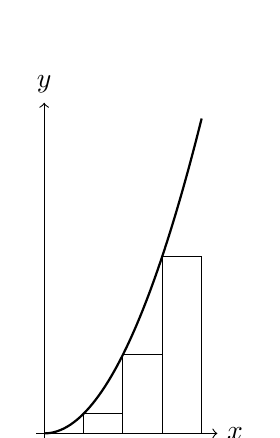
\begin{tikzpicture}[scale=1]
            \draw[->] (-0.1,0) -- (2.2,0) node[right] {$x$};
            \draw[->] (0,-0.1) -- (0,4.2) node[above] {$y$};
            \foreach \i in {0,...,3} {
                \pgfmathsetmacro{\xleft}{\i*0.5}
                \pgfmathsetmacro{\height}{\xleft*\xleft}
                \draw[black] (\xleft,0) rectangle ({\xleft+0.5}, {\height});
            }
            \draw[domain=0:2, smooth, variable=\x, thick] plot ({\x}, {\x*\x});
        \end{tikzpicture}
        \caption*{Left Endpoint}
    \end{minipage}
    \hfill
    \begin{minipage}{0.32\textwidth}
        \centering
        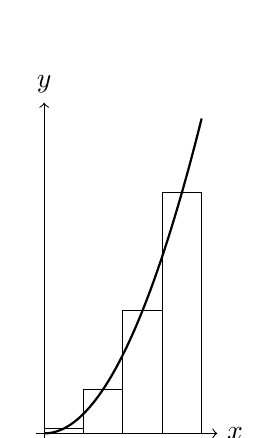
\begin{tikzpicture}[scale=1]
            \draw[->] (-0.1,0) -- (2.2,0) node[right] {$x$};
            \draw[->] (0,-0.1) -- (0,4.2) node[above] {$y$};
            \foreach \i in {0,...,3} {
                \pgfmathsetmacro{\xleft}{\i*0.5}
                \pgfmathsetmacro{\xmid}{\xleft + 0.25}
                \pgfmathsetmacro{\height}{\xmid*\xmid}
                \draw[black] (\xleft,0) rectangle ({\xleft+0.5}, {\height});
            }
            \draw[domain=0:2, smooth, variable=\x, thick] plot ({\x}, {\x*\x});
        \end{tikzpicture}
        \caption*{Midpoint}
    \end{minipage}
    \hfill
    \begin{minipage}{0.32\textwidth}
        \centering
        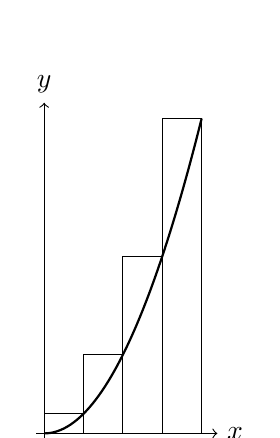
\begin{tikzpicture}[scale=1]
            \draw[->] (-0.1,0) -- (2.2,0) node[right] {$x$};
            \draw[->] (0,-0.1) -- (0,4.2) node[above] {$y$};
            \foreach \i in {0,...,3} {
                \pgfmathsetmacro{\xleft}{\i*0.5}
                \pgfmathsetmacro{\xright}{\xleft + 0.5}
                \pgfmathsetmacro{\height}{\xright*\xright}
                \draw[black] (\xleft,0) rectangle ({\xleft+0.5}, {\height});
            }
            \draw[domain=0:2, smooth, variable=\x, thick] plot ({\x}, {\x*\x});
        \end{tikzpicture}
        \caption*{Right Endpoint}
    \end{minipage}
\end{figure}
\subsubsection*{Trapezoidal Approximation}
\begin{figure}[H]
    \centering
    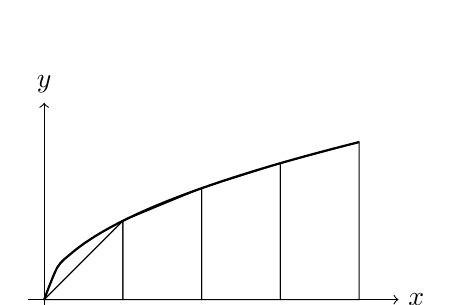
\begin{tikzpicture}[scale=1]
        \draw[->] (-0.2,0) -- (4.5,0) node[right] {$x$};
        \draw[->] (0,-0.2) -- (0,2.5) node[above] {$y$};
        \foreach \i in {0,...,3} {
            \pgfmathsetmacro{\xleft}{\i}
            \pgfmathsetmacro{\xright}{\xleft + 1}
            \pgfmathsetmacro{\yleft}{sqrt(\xleft)}
            \pgfmathsetmacro{\yright}{sqrt(\xright)}
            \draw[draw=black]
                (\xleft,0) -- (\xleft,\yleft) -- (\xright,\yright) -- (\xright,0) -- cycle;
        }
        \draw[domain=0:4, smooth, variable=\x, thick] plot ({\x}, {sqrt(\x)});
    \end{tikzpicture}
\end{figure}
If $f$ is continuous, the area under the curve of $f$ from $x=a$ to $x=b$ is:
\[
    \displaystyle
    \text{Area} \simeq\frac{b-a}{2n}\left[f(x_0)+2f(x_1)+\dots+2f(x_{n-1})+f(x_n)\right]
\]
\subsubsection{Area Under a Curve}
\begin{figure}[H]
    \centering
    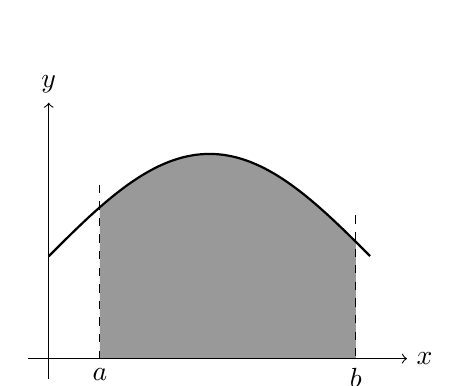
\begin{tikzpicture}[scale=1.3]
        \draw[->] (-0.2, 0) -- (3.5, 0) node[right] {$x$};
        \draw[->] (0, -0.2) -- (0, 2.5) node[above] {$y$};
        \draw[dashed] (.5,1.7) -- (.5,0) node[below]{$a$};
        \draw[dashed] (3,1.4) -- (3,0) node[below]{$b$};
        \begin{scope}
            \clip (.5,0) -- plot[domain=.5:3, smooth] (\x,{sin(\x r)+1}) -- (3,0) -- cycle;
            \fill[fill=black, opacity=.4] (0,0) rectangle (3.14,3);
        \end{scope}
        \draw[thick, black, domain=0:3.14, smooth, variable=\x] plot (\x,{sin(\x r)+1});
    \end{tikzpicture}
\end{figure}
The area under the graph of a continuous function $f(x)$ over the interval $[a, b]$ is given by the definite integral:
\[
    A = \int_a^b f(x)\,dx
\]
\noindent If $f(x) \geq 0$ on $[a, b]$, this integral gives the area between the curve and the $x$-axis. 
If $f(x)$ takes negative values, the integral represents \textbf{signed area}.
\subsubsection{Area Between Two Curves}


\section*{Proofs}
\addcontentsline{toc}{section}{Proofs}
\subsection{testing}
\end{document}
